% Options for packages loaded elsewhere
\PassOptionsToPackage{unicode}{hyperref}
\PassOptionsToPackage{hyphens}{url}
%
\documentclass[
]{article}
\usepackage{amsmath,amssymb}
\usepackage{iftex}
\ifPDFTeX
  \usepackage[T1]{fontenc}
  \usepackage[utf8]{inputenc}
  \usepackage{textcomp} % provide euro and other symbols
\else % if luatex or xetex
  \usepackage{unicode-math} % this also loads fontspec
  \defaultfontfeatures{Scale=MatchLowercase}
  \defaultfontfeatures[\rmfamily]{Ligatures=TeX,Scale=1}
\fi
\usepackage{lmodern}
\ifPDFTeX\else
  % xetex/luatex font selection
\fi
% Use upquote if available, for straight quotes in verbatim environments
\IfFileExists{upquote.sty}{\usepackage{upquote}}{}
\IfFileExists{microtype.sty}{% use microtype if available
  \usepackage[]{microtype}
  \UseMicrotypeSet[protrusion]{basicmath} % disable protrusion for tt fonts
}{}
\makeatletter
\@ifundefined{KOMAClassName}{% if non-KOMA class
  \IfFileExists{parskip.sty}{%
    \usepackage{parskip}
  }{% else
    \setlength{\parindent}{0pt}
    \setlength{\parskip}{6pt plus 2pt minus 1pt}}
}{% if KOMA class
  \KOMAoptions{parskip=half}}
\makeatother
\usepackage{xcolor}
\usepackage[margin=1in]{geometry}
\usepackage{graphicx}
\makeatletter
\def\maxwidth{\ifdim\Gin@nat@width>\linewidth\linewidth\else\Gin@nat@width\fi}
\def\maxheight{\ifdim\Gin@nat@height>\textheight\textheight\else\Gin@nat@height\fi}
\makeatother
% Scale images if necessary, so that they will not overflow the page
% margins by default, and it is still possible to overwrite the defaults
% using explicit options in \includegraphics[width, height, ...]{}
\setkeys{Gin}{width=\maxwidth,height=\maxheight,keepaspectratio}
% Set default figure placement to htbp
\makeatletter
\def\fps@figure{htbp}
\makeatother
\setlength{\emergencystretch}{3em} % prevent overfull lines
\providecommand{\tightlist}{%
  \setlength{\itemsep}{0pt}\setlength{\parskip}{0pt}}
\setcounter{secnumdepth}{-\maxdimen} % remove section numbering
\usepackage{newunicodechar}
\newunicodechar{Σ}{\ensuremath{\sum}}
\newunicodechar{√}{\ensuremath{\sqrt}}
\usepackage{booktabs}
\usepackage{longtable}
\usepackage{array}
\usepackage{multirow}
\usepackage{wrapfig}
\usepackage{float}
\usepackage{colortbl}
\usepackage{pdflscape}
\usepackage{tabu}
\usepackage{threeparttable}
\usepackage{threeparttablex}
\usepackage[normalem]{ulem}
\usepackage{makecell}
\usepackage{xcolor}
\ifLuaTeX
  \usepackage{selnolig}  % disable illegal ligatures
\fi
\IfFileExists{bookmark.sty}{\usepackage{bookmark}}{\usepackage{hyperref}}
\IfFileExists{xurl.sty}{\usepackage{xurl}}{} % add URL line breaks if available
\urlstyle{same}
\hypersetup{
  pdftitle={Supplementary data - Phonological Networks and Systematicity in Early Lexical Acquisition},
  pdfauthor={anonymised for review},
  hidelinks,
  pdfcreator={LaTeX via pandoc}}

\title{Supplementary data - Phonological Networks and Systematicity in
Early Lexical Acquisition}
\author{anonymised for review}
\date{}

\begin{document}
\maketitle

The supplementary materials below present further analyses and examples
from the main study. This data is included here for transparency and
further explanation. All scripts and data for our analysis can be found
on the project's GitHub page at
\url{https://github.com/cathelaing/PhonologicalNetworks}.

The analyses below (S1:S3) show:

\begin{itemize}
\tightlist
\item
  S1: Demonstration of how phonological distance was calculated with
  examples
\item
  S2: Correlations between age of production (AoP) and network
  connectivity
\item
  S3: Full model output tables from the analyses in the main paper
\end{itemize}

\hypertarget{s1-establishing-phonological-distance}{%
\subsubsection{S1: Establishing phonological
distance}\label{s1-establishing-phonological-distance}}

\begin{longtable}[t]{ccccccccc}
\caption{\label{tab:table-model-outputs}ADD}\\
\toprule
\multicolumn{1}{c}{ } & \multicolumn{2}{c}{col\_baby} & \multicolumn{3}{c}{col\_balloon} & \multicolumn{3}{c}{col\_sky} \\
\cmidrule(l{3pt}r{3pt}){2-3} \cmidrule(l{3pt}r{3pt}){4-6} \cmidrule(l{3pt}r{3pt}){7-9}
Word position & Consonant & Features & Consonant & Features & Sum squared differences & Consonant & Features & Sum squared differences\\
\midrule
S1C1 & b & -1,1,0,-1,1,1,0,-1,1,0,0 & b & -1,1,0,-1,1,1,0,-1,1,0,0 & 0+0+0+0+0+0+0+0+0+0+0 & s & -0.5,1,-1,-1,0,-1,1,-1,-1,1,0 & 0.25+0+1+0+1+4+1+0+4+1+0\\
S1C2 & - & 0 & - & 0 & - & k & -1,1,-1,-1,1,-1,-1,-1,-1,-1,0 & 1+1+1+1+1+1+1+1+1+1+0\\
S2C1 & b & -1,1,0,-1,1,1,0,-1,1,0,0 & l & 0.5,0,1,0,-1,-1,1,-1,-1,1,0 & 2.25+1+1+1+4+4+1+0+4+1+0 & - & 0 & 1+1+0+1+1+1+0+1+1+0+0\\
SFC1 & - & 0 & n & 0,0,1,1,1,-1,1,-1,-1,1,0 & 0+0+1+1+1+1+1+1+1+1+0 & - & 0 & -\\
Phonological distance (Σ √(sum squared differences)) & NA & NA & NA & NA & 7.21590931844225 & NA & NA & 9.30802897123297\\
\bottomrule
\end{longtable}

\hypertarget{s2-age-of-production-aop-connectivity}{%
\subsubsection{S2: Age of production (AoP) \textasciitilde{}
connectivity}\label{s2-age-of-production-aop-connectivity}}

\begin{longtable}[t]{cccc}
\caption{\label{tab:table-aop-deg-corr}Outputs (rho and p values) of AoP-degree Spearman's correlation tests for each infant in the dataset.}\\
\toprule
Speaker & Corpus & rho & p\\
\midrule
Alex & English & -0.20 & <0.001\\
Lily & English & -0.24 & <0.001\\
Naima & English & -0.27 & <0.001\\
Violet & English & -0.23 & <0.001\\
William & English & -0.21 & <0.001\\
\addlinespace
Anais & French & -0.02 & 0.593\\
Marie & French & -0.18 & <0.001\\
Nathan & French & -0.11 & 0.045\\
Tim & French & -0.21 & <0.001\\
\bottomrule
\end{longtable}

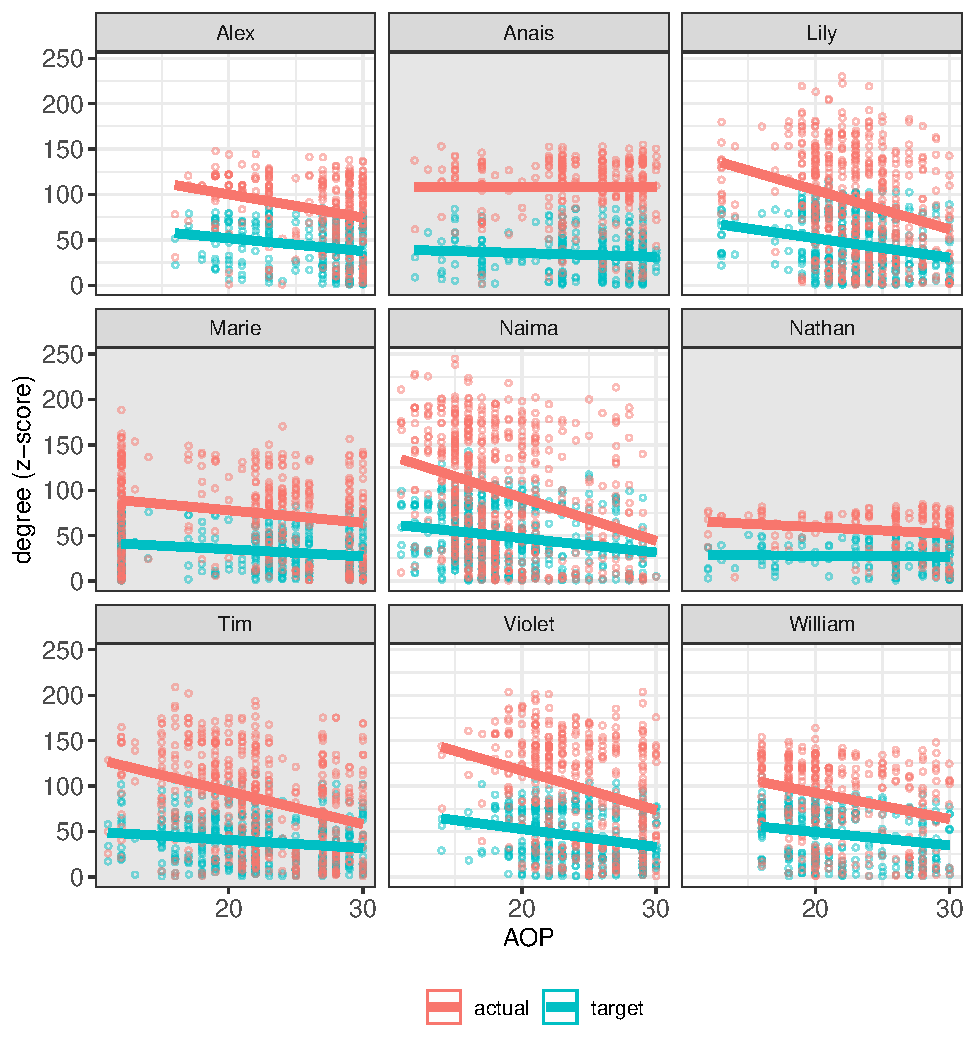
\includegraphics{PhonNetworksSupplementaryData_files/figure-latex/Figure-AOP-deg-corr-1.pdf}

\newpage

\hypertarget{s3-network-growth-models-full-model-outputs}{%
\subsubsection{S3: Network growth models: Full model
outputs}\label{s3-network-growth-models-full-model-outputs}}

\end{document}
